\subsection{Gedarg ondezoek}
Voor het gedrag van de bijen te kunnen verwezelijken naar een software achtige structuur, is er gebruik gemaakt van
\cite{akbari_mohammadi_ziarati_2010}. In dit artikel staat een numerieke beschrijving van het gedrag van bijen.
Hierbij worden de verschillende rollen en acties die deze dieren uit kunnen voeren beschreven
en de interpetatie voor dit project hiervan zal in dit hoofdstuk beschreven worden.

\subsubsection{Werkrollen}
In het artikel worden over verschillende rollen die de bijen kunnen aannemen namelijk; werkeloos, werkend en scouting.
Een werkelozen bij kan twee acties ondernemen, gaan scouten naar eten afvankelijk van de hoeveelheid bijen die nog aanwezig zijn in de korf,
of wachten tot hij word geroepen door een werkende bij. Een scoutende bij is op zoek naar eten buiten de bijenkorf en veranderd naar een werkende bij
wanneer hij dit eten heeft gevonden en terug gaat brengen naar de bijenkorf.\\

Een werkende bij is bezig met het halen van het voedsel, maar kan hierbij ook nog keuzes maken geraleerd met hoe goed het eten is dat hij heeft gevonden.
De waarde van dit eten wordt later op terug gekomen. Voornu is het belangrijk dat wanneer er veel eten is dan kan de werkende bij 'dansen'
om werkelozen bijen mee te nemen naar het eten. Wanneer er niet veel eten meer over is dan zal de bij niet meer dansen en direct terug gaan naar de voedselbron 
in zen eentje.

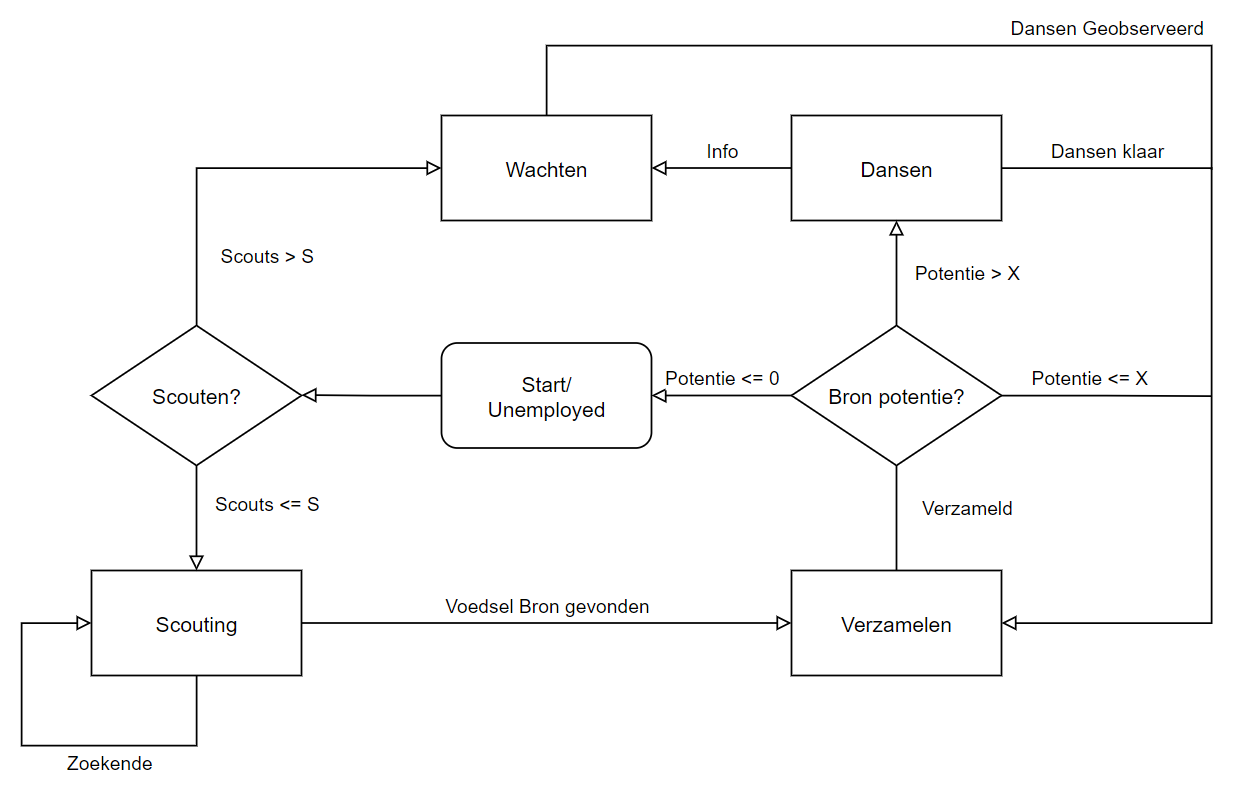
\includegraphics[scale=0.33]{../IMAGES/BijengedragFlowchart.png}

